\documentclass[border=15pt]{standalone}
\usepackage{amsmath, amssymb}
\usepackage{tikz}

\definecolor{ptcol}{HTML}{E53935}
\definecolor{lncol}{HTML}{1E88E5}

\begin{document}
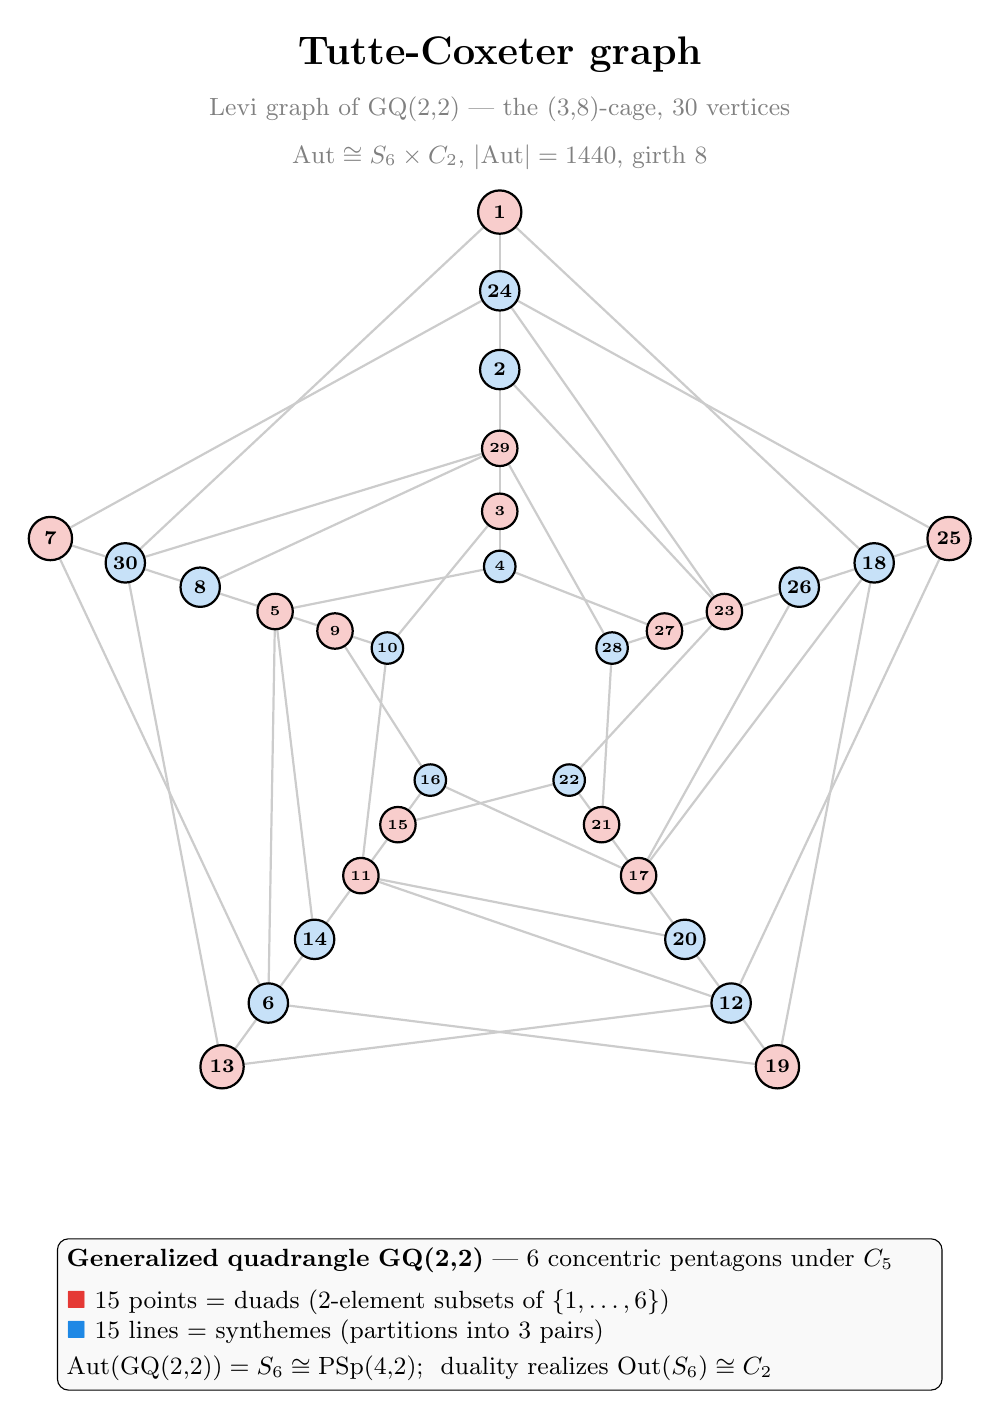
\begin{tikzpicture}[
  edge/.style={thick, gray!40},
  title/.style={font=\Large\bfseries},
  subtitle/.style={font=\small, text=gray},
]

\node[title] at (0, 8.0) {Tutte-Coxeter graph};
\node[subtitle] at (0, 7.3) {Levi graph of $\mathrm{GQ}(2{,}2)$ --- the $(3{,}8)$-cage, 30 vertices};
\node[subtitle] at (0, 6.7) {$\mathrm{Aut} \cong S_6 \times C_2$, $|\mathrm{Aut}| = 1440$, girth $8$};

\coordinate (p1) at (0.0000, 6.0000);
\coordinate (p2) at (0.0000, 4.0000);
\coordinate (p3) at (0.0000, 2.2000);
\coordinate (p4) at (0.0000, 1.5000);
\coordinate (p5) at (-2.8532, 0.9271);
\coordinate (p6) at (-2.9389, -4.0451);
\coordinate (p7) at (-5.7063, 1.8541);
\coordinate (p8) at (-3.8042, 1.2361);
\coordinate (p9) at (-2.0923, 0.6798);
\coordinate (p10) at (-1.4266, 0.4635);
\coordinate (p11) at (-1.7634, -2.4271);
\coordinate (p12) at (2.9389, -4.0451);
\coordinate (p13) at (-3.5267, -4.8541);
\coordinate (p14) at (-2.3511, -3.2361);
\coordinate (p15) at (-1.2931, -1.7798);
\coordinate (p16) at (-0.8817, -1.2135);
\coordinate (p17) at (1.7634, -2.4271);
\coordinate (p18) at (4.7553, 1.5451);
\coordinate (p19) at (3.5267, -4.8541);
\coordinate (p20) at (2.3511, -3.2361);
\coordinate (p21) at (1.2931, -1.7798);
\coordinate (p22) at (0.8817, -1.2135);
\coordinate (p23) at (2.8532, 0.9271);
\coordinate (p24) at (0.0000, 5.0000);
\coordinate (p25) at (5.7063, 1.8541);
\coordinate (p26) at (3.8042, 1.2361);
\coordinate (p27) at (2.0923, 0.6798);
\coordinate (p28) at (1.4266, 0.4635);
\coordinate (p29) at (0.0000, 3.0000);
\coordinate (p30) at (-4.7553, 1.5451);

\draw[edge] (p1) -- (p2);
\draw[edge] (p1) -- (p30);
\draw[edge] (p1) -- (p18);
\draw[edge] (p2) -- (p3);
\draw[edge] (p2) -- (p23);
\draw[edge] (p3) -- (p4);
\draw[edge] (p3) -- (p10);
\draw[edge] (p4) -- (p27);
\draw[edge] (p4) -- (p5);
\draw[edge] (p5) -- (p14);
\draw[edge] (p5) -- (p6);
\draw[edge] (p6) -- (p19);
\draw[edge] (p6) -- (p7);
\draw[edge] (p7) -- (p24);
\draw[edge] (p7) -- (p8);
\draw[edge] (p8) -- (p9);
\draw[edge] (p8) -- (p29);
\draw[edge] (p9) -- (p10);
\draw[edge] (p9) -- (p16);
\draw[edge] (p10) -- (p11);
\draw[edge] (p11) -- (p20);
\draw[edge] (p11) -- (p12);
\draw[edge] (p12) -- (p25);
\draw[edge] (p12) -- (p13);
\draw[edge] (p13) -- (p30);
\draw[edge] (p13) -- (p14);
\draw[edge] (p14) -- (p15);
\draw[edge] (p15) -- (p22);
\draw[edge] (p15) -- (p16);
\draw[edge] (p16) -- (p17);
\draw[edge] (p17) -- (p18);
\draw[edge] (p17) -- (p26);
\draw[edge] (p18) -- (p19);
\draw[edge] (p19) -- (p20);
\draw[edge] (p20) -- (p21);
\draw[edge] (p21) -- (p28);
\draw[edge] (p21) -- (p22);
\draw[edge] (p22) -- (p23);
\draw[edge] (p23) -- (p24);
\draw[edge] (p24) -- (p25);
\draw[edge] (p25) -- (p26);
\draw[edge] (p26) -- (p27);
\draw[edge] (p27) -- (p28);
\draw[edge] (p28) -- (p29);
\draw[edge] (p29) -- (p30);

\node[circle, draw, thick, fill=ptcol!25, minimum size=5.5mm, inner sep=0pt, font=\scriptsize\bfseries] at (0.0000, 6.0000) {1};
\node[circle, draw, thick, fill=lncol!25, minimum size=5mm, inner sep=0pt, font=\scriptsize\bfseries] at (0.0000, 4.0000) {2};
\node[circle, draw, thick, fill=ptcol!25, minimum size=4.5mm, inner sep=0pt, font=\tiny\bfseries] at (0.0000, 2.2000) {3};
\node[circle, draw, thick, fill=lncol!25, minimum size=4mm, inner sep=0pt, font=\tiny\bfseries] at (0.0000, 1.5000) {4};
\node[circle, draw, thick, fill=ptcol!25, minimum size=4.5mm, inner sep=0pt, font=\tiny\bfseries] at (-2.8532, 0.9271) {5};
\node[circle, draw, thick, fill=lncol!25, minimum size=5mm, inner sep=0pt, font=\scriptsize\bfseries] at (-2.9389, -4.0451) {6};
\node[circle, draw, thick, fill=ptcol!25, minimum size=5.5mm, inner sep=0pt, font=\scriptsize\bfseries] at (-5.7063, 1.8541) {7};
\node[circle, draw, thick, fill=lncol!25, minimum size=5mm, inner sep=0pt, font=\scriptsize\bfseries] at (-3.8042, 1.2361) {8};
\node[circle, draw, thick, fill=ptcol!25, minimum size=4.5mm, inner sep=0pt, font=\tiny\bfseries] at (-2.0923, 0.6798) {9};
\node[circle, draw, thick, fill=lncol!25, minimum size=4mm, inner sep=0pt, font=\tiny\bfseries] at (-1.4266, 0.4635) {10};
\node[circle, draw, thick, fill=ptcol!25, minimum size=4.5mm, inner sep=0pt, font=\tiny\bfseries] at (-1.7634, -2.4271) {11};
\node[circle, draw, thick, fill=lncol!25, minimum size=5mm, inner sep=0pt, font=\scriptsize\bfseries] at (2.9389, -4.0451) {12};
\node[circle, draw, thick, fill=ptcol!25, minimum size=5.5mm, inner sep=0pt, font=\scriptsize\bfseries] at (-3.5267, -4.8541) {13};
\node[circle, draw, thick, fill=lncol!25, minimum size=5mm, inner sep=0pt, font=\scriptsize\bfseries] at (-2.3511, -3.2361) {14};
\node[circle, draw, thick, fill=ptcol!25, minimum size=4.5mm, inner sep=0pt, font=\tiny\bfseries] at (-1.2931, -1.7798) {15};
\node[circle, draw, thick, fill=lncol!25, minimum size=4mm, inner sep=0pt, font=\tiny\bfseries] at (-0.8817, -1.2135) {16};
\node[circle, draw, thick, fill=ptcol!25, minimum size=4.5mm, inner sep=0pt, font=\tiny\bfseries] at (1.7634, -2.4271) {17};
\node[circle, draw, thick, fill=lncol!25, minimum size=5mm, inner sep=0pt, font=\scriptsize\bfseries] at (4.7553, 1.5451) {18};
\node[circle, draw, thick, fill=ptcol!25, minimum size=5.5mm, inner sep=0pt, font=\scriptsize\bfseries] at (3.5267, -4.8541) {19};
\node[circle, draw, thick, fill=lncol!25, minimum size=5mm, inner sep=0pt, font=\scriptsize\bfseries] at (2.3511, -3.2361) {20};
\node[circle, draw, thick, fill=ptcol!25, minimum size=4.5mm, inner sep=0pt, font=\tiny\bfseries] at (1.2931, -1.7798) {21};
\node[circle, draw, thick, fill=lncol!25, minimum size=4mm, inner sep=0pt, font=\tiny\bfseries] at (0.8817, -1.2135) {22};
\node[circle, draw, thick, fill=ptcol!25, minimum size=4.5mm, inner sep=0pt, font=\tiny\bfseries] at (2.8532, 0.9271) {23};
\node[circle, draw, thick, fill=lncol!25, minimum size=5mm, inner sep=0pt, font=\scriptsize\bfseries] at (0.0000, 5.0000) {24};
\node[circle, draw, thick, fill=ptcol!25, minimum size=5.5mm, inner sep=0pt, font=\scriptsize\bfseries] at (5.7063, 1.8541) {25};
\node[circle, draw, thick, fill=lncol!25, minimum size=5mm, inner sep=0pt, font=\scriptsize\bfseries] at (3.8042, 1.2361) {26};
\node[circle, draw, thick, fill=ptcol!25, minimum size=4.5mm, inner sep=0pt, font=\tiny\bfseries] at (2.0923, 0.6798) {27};
\node[circle, draw, thick, fill=lncol!25, minimum size=4mm, inner sep=0pt, font=\tiny\bfseries] at (1.4266, 0.4635) {28};
\node[circle, draw, thick, fill=ptcol!25, minimum size=4.5mm, inner sep=0pt, font=\tiny\bfseries] at (0.0000, 3.0000) {29};
\node[circle, draw, thick, fill=lncol!25, minimum size=5mm, inner sep=0pt, font=\scriptsize\bfseries] at (-4.7553, 1.5451) {30};

\node[draw, rounded corners, fill=gray!5,
  text width=11cm, align=left, font=\small]
  at (0, -8.0) {
  \textbf{Generalized quadrangle GQ(2,2)} --- 6 concentric pentagons under $C_5$ \\[4pt]
  \textcolor{ptcol}{$\blacksquare$} 15 points = duads (2-element subsets of $\{1,\ldots,6\}$) \\
  \textcolor{lncol}{$\blacksquare$} 15 lines = synthemes (partitions into 3 pairs) \\[2pt]
  $\mathrm{Aut}(\mathrm{GQ}(2{,}2)) = S_6 \cong \mathrm{PSp}(4{,}2)$; \ 
  duality realizes $\mathrm{Out}(S_6) \cong C_2$
};

\end{tikzpicture}
\end{document}